% =====================================================================
% Figure 2 — Cam lift schematic (TikZ + pgfplots)
% Shows the two critical points of the cam profile (positive accel
% peak and deceleration peak), reconstructed analytically from the
% cam dimensioning of the AP 1.8 head.
% =====================================================================

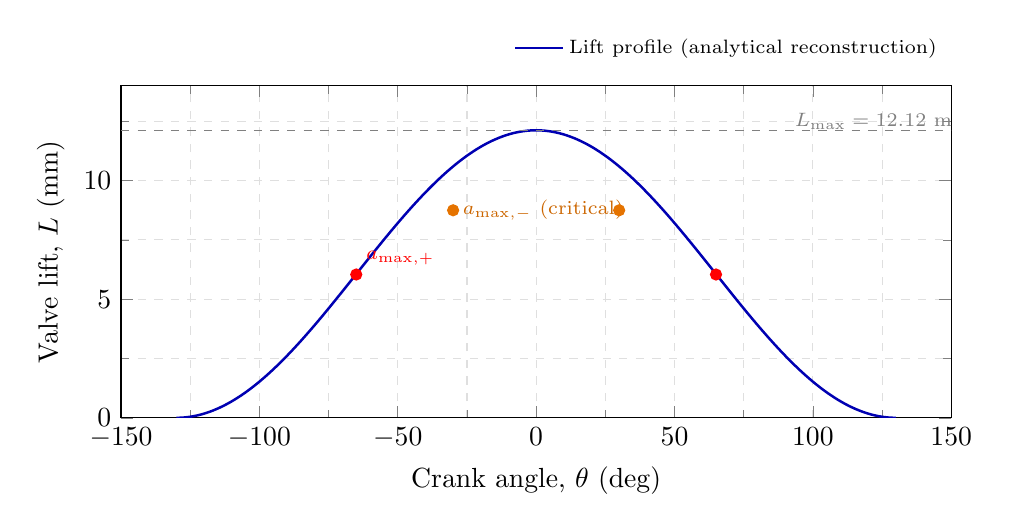
\begin{tikzpicture}
  \begin{axis}[
    width=\linewidth,
    height=5.8cm,
    xlabel={Crank angle, $\theta$ (deg)},
    ylabel={Valve lift, $L$ (mm)},
    xmin=-150, xmax=150,
    ymin=0,    ymax=14,
    grid=both,
    grid style={dashed,gray!25},
    minor tick num=1,
    legend style={
      at={(1,1.05)}, anchor=south east,
      font=\scriptsize, draw=none, fill=none,
      legend columns=-1,
    },
  ]
  % Smooth bell-shaped lift curve (analytical reconstruction).
  % Peak lift L_max = 12.12 mm at theta = 0 deg.
  \addplot[blue!70!black, line width=0.9pt, smooth, samples=200, domain=-130:130]
    {12.12 * (cos(deg(pi*x/260)))^2};
  \addlegendentry{Lift profile (analytical reconstruction)}

  % Critical point 1: positive acceleration peak (L+ = 6.04 mm)
  \addplot[red, mark=*, mark size=2.0pt, only marks] coordinates {(-65, 6.04)};
  \node[anchor=south west, red, font=\scriptsize] at (axis cs:-65,6.04) {$a_{\max,+}$};

  % Critical point 2: deceleration peak (L- = 8.747 mm)
  \addplot[orange!90!black, mark=*, mark size=2.0pt, only marks] coordinates {(-30, 8.747)};
  \node[anchor=west, orange!80!black, font=\scriptsize] at (axis cs:-30,8.747) {$a_{\max,-}$ (critical)};

  % Symmetric points on closing side
  \addplot[red,        mark=*, mark size=2.0pt, only marks] coordinates {( 65, 6.04)};
  \addplot[orange!90!black, mark=*, mark size=2.0pt, only marks] coordinates {( 30, 8.747)};

  % L_max line
  \addplot[gray, dashed] coordinates {(-150,12.12) (150,12.12)};
  \node[anchor=west, gray, font=\scriptsize] at (axis cs:90,12.5) {$L_{\max}=12.12$ mm};

  \end{axis}
\end{tikzpicture}
